%%%%% Literature Review %%%%%
\section{Literature Review} 
In the last two decades, significant progress in electronic and computer technologies has led to remarkable 
growth in the field of manipulator robotics. Manipulators developed by various institutions have been integrated 
into the industrial sector to autonomously or semi-autonomously perform repetitive tasks. Simultaneously, 
manipulators are utilized for tasks with stringent precision requirements to minimize errors. Additionally, 
essential tasks are undertook by manipulators to substitute for humans in challenging environments. 
\subsection{Manipulators in Biology Field}
With a growing emphasis on the field of biology, manipulators have also been introduced to provide assistance. 
In the field of medicine, manipulators have been utilized since the end of the last century. The AESOP robotic 
surgical system, proposed by Computer Motion founded by Yulun Wang in 1993, was investigated in laparoscopic 
surgery in 1997 \cite{AESOP}. Afterward, the ZEUS robotic surgical system endowed with a trilateral manipulator 
configuration was proposed by Computer Motion in 1998 \cite{ZEUS}.During the period from 1999 to 2001, the ZEUS 
system was utilized for a series of clinical surgeries, demonstrating excellent performance 
\cite{ZEUS_example1,ZEUS_example2,ZEUS_example3}. At the beginning of the 21st century, a novel 
robotic system, da Vinci robotic surgery system, was designed to facilitate more intricate surgical procedures 
\cite{da_Vinci}. Moreover, manipulators can be leveraged in the field of biological physics as a viable approach 
for biological experiments. In the HIFU system developed by An et al., the SCARA (self compliant automatic robot 
assembly) robot was employed as manipulator, incorporating an ultrasound probe for the purpose of scanning 
biological tissues \cite{HIFU2017}. The robotic system FUSBOTs (Focal Ultrasound Surgery RoBOTs) was proposed 
and upgraded to accomplish more precise targeted treatment with multiple DoF (Degrees of Freedom) manipulators 
\cite{FUSBOT,FUSBOT_example1,FUSBOT_example2}. Despite the various utilization of manipulator platforms 
designed for accommodating ultrasonic transducers \cite{6DOF_HIFU,6DOF_HIFU_comp,6DOF_HIFU_ABB}, 
certain limitations persist. Hence, a comparison of different manipulators is necessary in selection of appropriate 
type manipulator for integrating ultrasonic transducer. 

\subsection{Types of Manipulator}
From the perspective of geometry, rigid-body manipulators can be categorized into two main types: serial link and 
parallel mechanisms \cite{MECH0089book}. The control of parallel mechanisms is relatively complex. Meanwhile, 
serial link manipulators can be further divided into five types: articulated (RRR), spherical (RRP), SCARA (RRP), 
cylindrical (RPP), or Cartesian (PPP). Additionally, with the advancement of robotics technology, two other types 
of manipulators, namely serpentine and anthropomorphic, have demonstrated their advantages 
\cite{manipulators_types1,manipulators_types2}.
The comparative analysis will be conducted to highlight the distinctive features of different manipulators 
presented in Table \ref{tab:different_types_manipulators}, leading to the identification of the most suitable 
type for specific applications.
\begin{center}
    \begin{longtable}{l l l l}
    \caption{The Characteristics of Different Manipulators.} \label{tab:different_types_manipulators} \\
    \hline \multicolumn{1}{c}{\textbf{Manipulators}} & 
    \multicolumn{1}{c}{\textbf{Types}} & 
    \multicolumn{1}{c}{\textbf{DoF}} & 
    \multicolumn{1}{c}{\textbf{Features}} \\ \hline 
    \endfirsthead
    \multicolumn{4}{c}%
    {{\bfseries \tablename\ \thetable{} -- continued from previous page}} \\
    \hline \multicolumn{1}{c}{\textbf{Manipulators}} & 
    \multicolumn{1}{c}{\textbf{Types}} & 
    \multicolumn{1}{c}{\textbf{DoF}} & 
    \multicolumn{1}{c}{\textbf{Features}} \\ \hline 
    \endhead
    \hline \multicolumn{4}{|r|}{{Continued on next page}} \\ \hline
    \endfoot
    \hline \hline
    \endlastfoot
    % table context
    \multirow{2}{*}{3D cartesian/gantry manipulator} & PPP & 3 & 1   \\
    & & & \\ \hline
    % \multirow{2}{*}{3D cartesian/gantry manipulator} & PPP & 3 & 1   \\
    % & & & \\ \hline
    \end{longtable}
\end{center}


\subsection{Working Principles}
Continuum robot can be broadly divided into two parts: a continuous bending structure and a fixed base containing actuating and 
controlling devices.\\
The continuous bending structure can be seen as the working arm of the robot. A flexible backbone shapes the arm, and it can be rotated 
and bent by dragging/releasing the different cables (tendons) around it. 
When the joystick in the fixed base is manipulated manually, the programmed stepper motor will step forward/backward by the 
corresponding number of steps. These motors are connected to different cables located in the bending structure (arm), the motors 
dragging the cables, thereby making cable contract. Finally, the contraction of different cables will rotate and bend the backbone, 
which is the core component of the arm, thereby changing the posture of the arm.\\
This process can be likened to the movement of the human arms. cables can be understood as tendons/muscle bundles and backbone as 
the main skeleton.
\begin{figure}[H] %[H] "corresponds to start the figure Here" 
    \centering %alignment can be flushleft or flushright
    \captionsetup{labelsep=colon}
    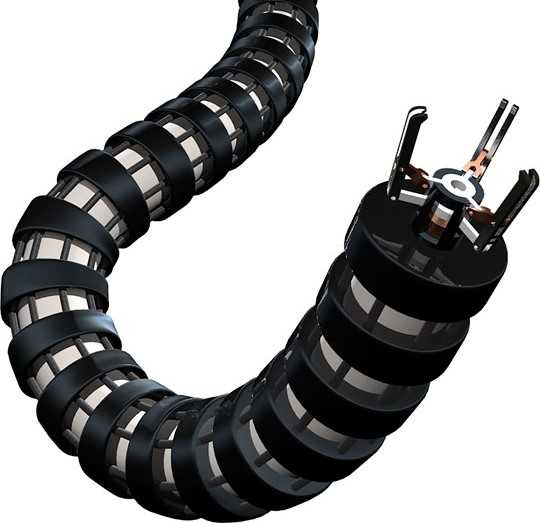
\includegraphics[width=.8\textwidth]{Image/LR/CR_example.jpg} 
    \caption[An example of continuum robot]
    {\centering \textit{\textbf{An example of continuum robot }}\cite{CR_example}.}
    \label{fig:CR_example}
\end{figure}
\noindent Different types of continuum robots have different backbones, actuating and flexible components, but they are generally all 
work under the same working principle stated above. \\
\subsection{Types of Continuum Robots}
Nowadays, a variety of continuum robots exist, each exhibiting unique structures and functions. They serve in different fields 
such as medicine, construction, and exploration. In this section, some of the most popular continuum robots will be introduced, 
providing basic insights into their structures as well as discussing their merits and drawbacks. \\
\subsubsection{Tendon-Driven Robots}
The arm of the Tendon-Driven robot consists of a backbone, several tendons and disks. The backbone defines the structure and 
posture of the entire robot arm, while disks define the diameter and divide the robot arm into segments, and tendons are 
stretched to create deformation and movements of different directions for the robot arm. \\
\begin{figure}[H] %[H] "corresponds to start the figure Here" 
    \centering %alignment can be flushleft or flushright
    \captionsetup{labelsep=colon}
    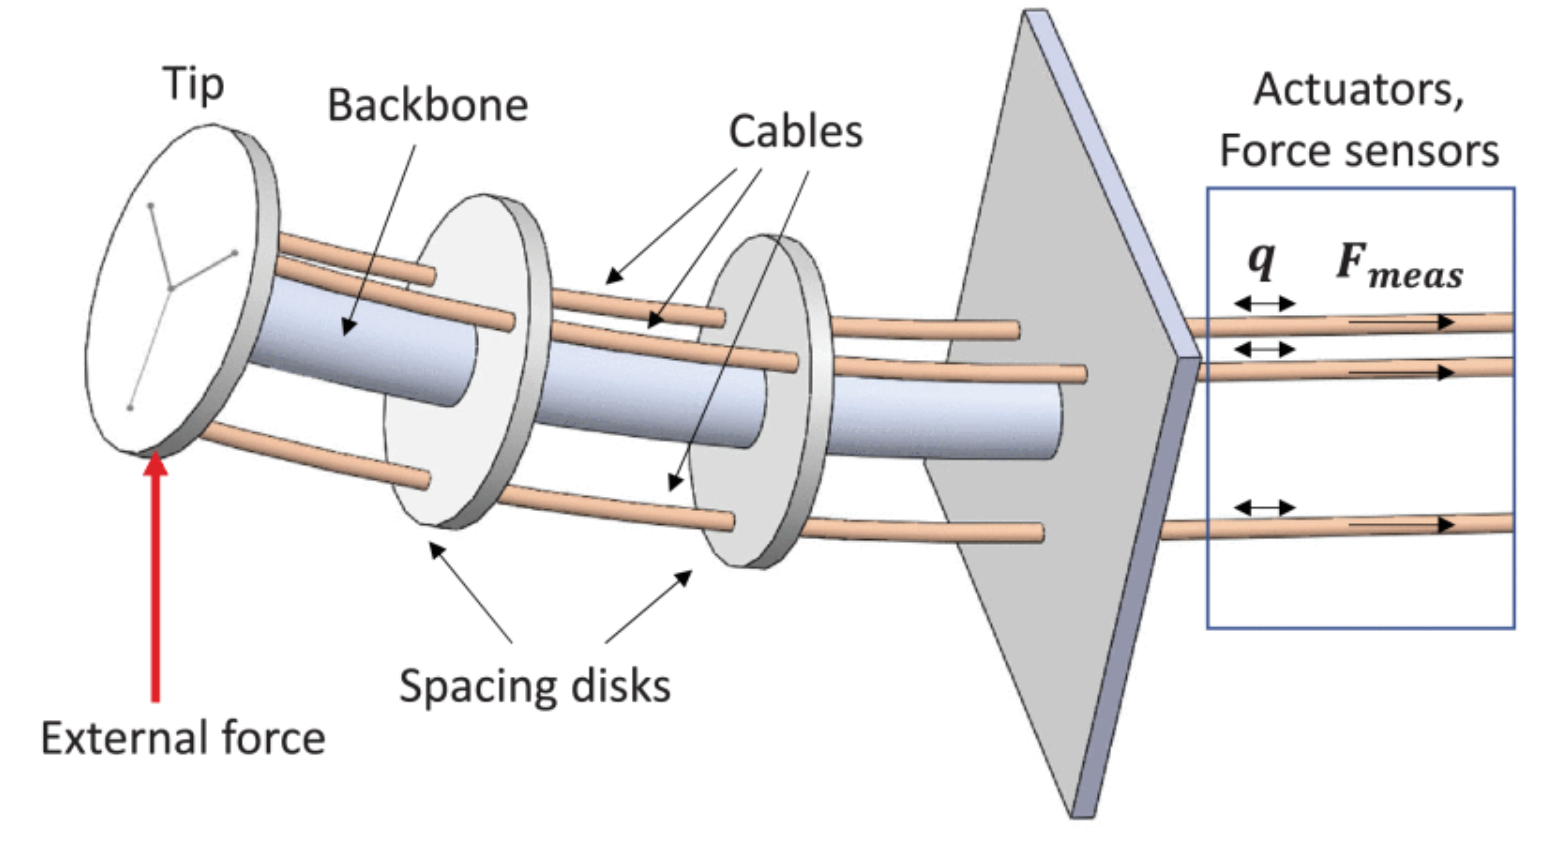
\includegraphics[width=.9\textwidth]{Image/LR/3tendon_1segment_CR.PNG} 
    \caption[The three tendons continuum robot with one segment]
    {\centering \textit{\textbf{The three tendons continuum robot with one segment}} \cite{3tendon_1segment_CR}.}
    \label{fig:3tendon_1segment_CR}
\end{figure}
\noindent Figure \ref{fig:3tendon_1segment_CR} shows only the simplest tenon-driven robots. In practical applications, there 
may be more than one backbone, and the disks are not necessarily parallel. \\
Compared with other continuum robots, one of the most significant advantages of tendon-driven robots is their flexibility. 
This advantage makes it more effective in performing tasks in complex and restrictive Spaces. In addition, due to the simple 
components needed to construct the robot, it is easier to meet lightweight design specifications. Moreover, like the 
concentric-tube continuum robots, tendon-driven continuum robots can be built designed on a small scale with diameters of 
below 10mm \cite{amanov2021tendon}. \\
However, due to its simple actuating principle, more complex algorithms are needed to control it more accurately. Also, the 
tendon-driven robots actuate by pulling the tendon, which makes the friction between the tendon and other components inevitable, 
which will accelerate the wearing speed of the tendon-driven robots.
\subsubsection{Fishbone Robots}
The fishbone robots are inspired by fishbones. It is comprised of multiple "fishbone units" which consist of rigid cross-shaped 
plates and soft rubber sleeves, with a layer of manganese alloy steel elastic plate embedded in the middle to form a rigid-soft 
coupled structure\cite{fishboneCR}. In contract to the existing single-backbone continuum robots, the middle backbone of the 
continuum robot is serially formed by multiple cross- arranged bioinspired fishbone units.  The fishbone units stack layer by 
layer, forming a spine-like shaper. Like tendon-driven robots, it utilizes cables to simulate muscle movement, causing layers 
of fishbones to bend in corresponding directions through cable stretching at different positions. 
\begin{figure}[H] %[H] "corresponds to start the figure Here" 
    \centering %alignment can be flushleft or flushright
    \captionsetup{labelsep=colon}
    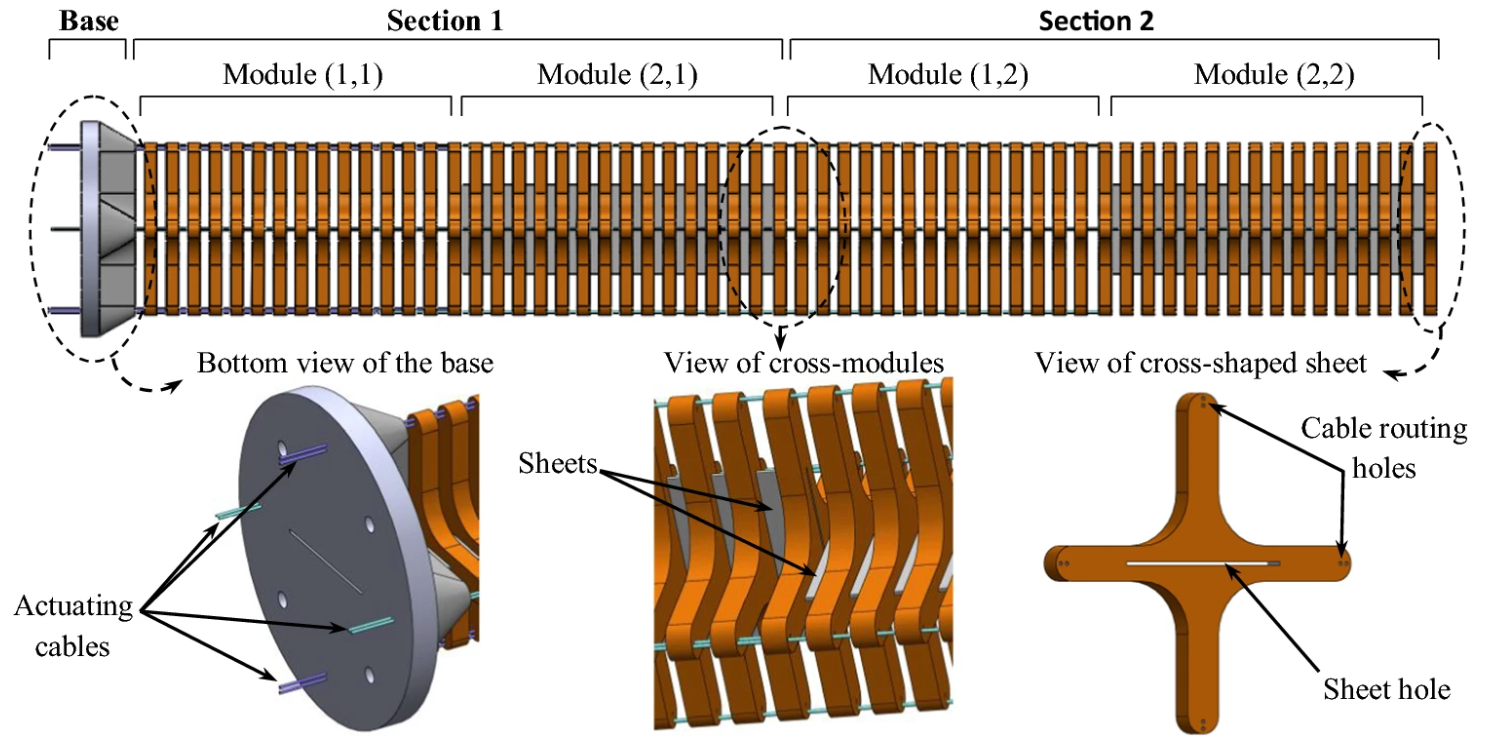
\includegraphics[width=.9\textwidth]{Image/LR/fishbone_CR_amouri2023bio.PNG} 
    \caption[The cable-driven fish bone continuum robot]
    {\centering \textit{\textbf{The cable-driven fish bone continuum robot with cable arrangement}} \cite{amouri2023bio}.}
    \label{fig:fishboneCR_2023bio}
\end{figure}
\noindent Because many fishbone units are stacked together as the backbone of the fishbone continuum robots, the structural 
stability of this kind of robot is very strong. The disadvantage, however, is that it is difficult to make lightweight designs 
since the density of the components is high.
\subsubsection{Concentric Tube Continuum Robots}
concentric tube robots, shaped like retractable walking sticks, consist of many tubes with decreasing diameters. Each tube is 
nested on top of the previous wider tube.  \\
The concentric robots are made of two parts: tubes and coaxial actuation units. The tubes are the main structural element of 
this robot and act as the backbone. The coaxial actuation unit consists of two motors which are responsible for rotation and 
translation movement respectively. Each tube is actuated by an independent coaxial actuation unit. 
\begin{figure}[H] %[H] "corresponds to start the figure Here" 
    \centering %alignment can be flushleft or flushright
    \captionsetup{labelsep=colon}
    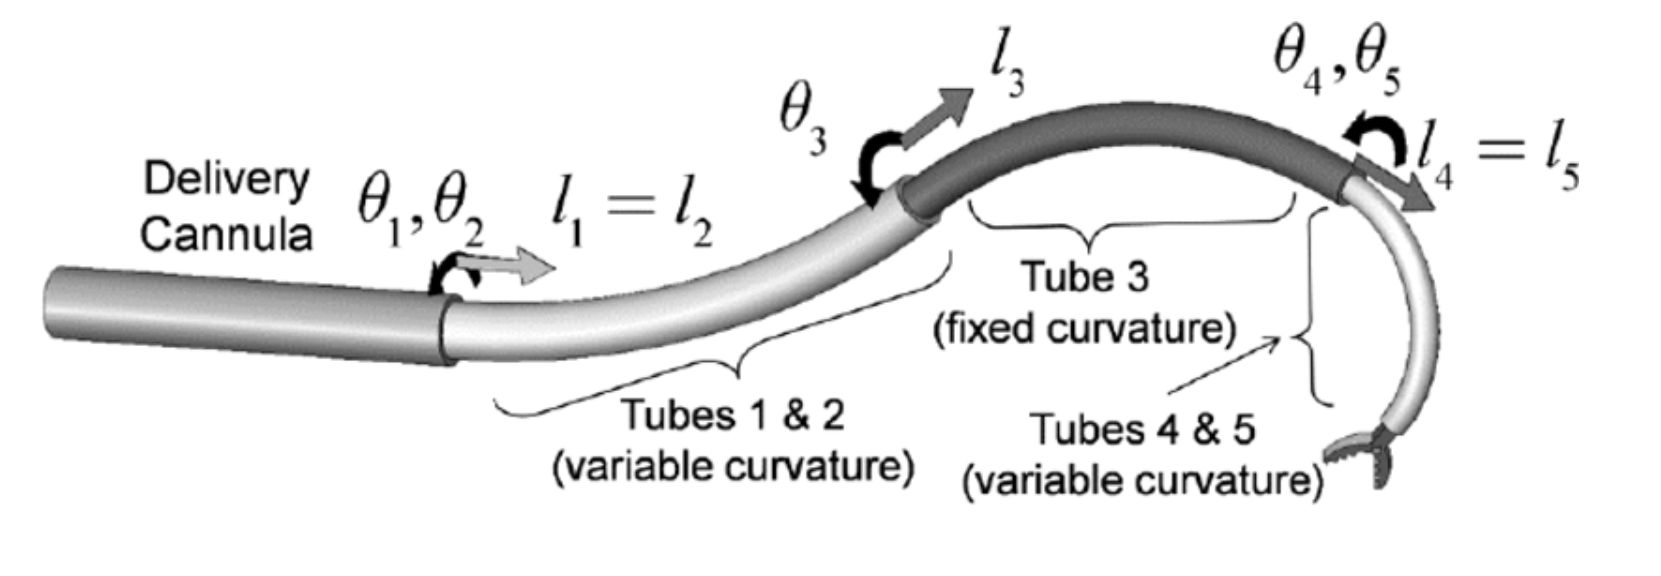
\includegraphics[width=.9\textwidth]{Image/LR/concentric_tube_CR.PNG} 
    \caption[An example concentric tube continuum robot]
    {\centering \textit{\textbf{An example concentric tube continuum robot}} \cite{CTCR_example}.}
    \label{fig:CTCR_example}
\end{figure}
\noindent The most significant advantage of this kind of robots is that of all the continuum robots, concentric tube robots have the 
smallest possible outer diameter and are best suited to work in confined and narrow Spaces. Therefore, it is the ideal choice 
for surgical operations. \\
Their disadvantages, on the other hand, are also very evident. Since each tube requires an independent actuation unit, the 
overall length of the robot cannot be very long, because longer lengths will lead to more tubes, and will lead to more tip 
position errors.



% change to new page
\newpage